\documentclass{article}
\usepackage[T1]{fontenc}
\usepackage{lmodern}
\usepackage{graphicx}
\usepackage{amsmath,amssymb}
\usepackage[a4paper,margin=2cm]{geometry}
\usepackage[absolute,overlay]{textpos}
\setlength{\TPHorizModule}{1mm}
\setlength{\TPVertModule}{1mm}
\usepackage[indonesian]{babel}
\usepackage{hyperref}
\setlength{\emergencystretch}{2em}
% unit: Halaman 84

\begin{document}

% === Halaman 84 (python/native) ===

• Column round menerapkan QR(a, b, c, d) kepada tiap kolom matriks state 4×4, 

sedangkan row round menerapkannya kepada tiap baris matriks. 

   // Column round

         QR( 0,  4,  8, 12) // kolom 1

         QR( 5,  9, 13,  1) // kolom 2

         QR(10, 14,  2,  6) // kolom 3

         QR(15,  3,  7, 11) // kolom 4

    // Row round

        QR( 0,  1,  2,  3) 

   // baris 1

        QR( 5,  6,  7,  4) 

   // baris 2

        QR(10, 11,  8,  9)    // baris 3

        QR(15, 12, 13, 14)   // baris 4

84

\#define ROTL(a,b) (((a) << (b)) | ((a) >> (32 - (b))))

\#define QR(a, b, c, d)( 



b \textasciicircum{}= ROTL(a + d, 7), \textbackslash{} 


c \textasciicircum{}= ROTL(b + a, 9), \textbackslash{} 


d \textasciicircum{}= ROTL(c + b,13), \textbackslash{} 


a \textasciicircum{}= ROTL(d + c,18))

QR(a, b, c, d):

      b  b  (a + d) <<<  7;

      c  c   (b + a) <<<  9;

      d  d  (c + b) <<< 13;

      a  a  (d + c) <<< 18;

% deskripsi: gambar native xref 321
\noindent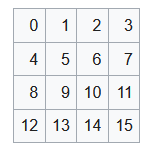
\includegraphics[width=0.85\textwidth]{../../images/python/page_084_img_01.png}

\end{document}
